\input{../preamble}
\input{../usercommands}

\begin{document}

\vspace*{2cm}

{\centerline{\bf\huge AST1100 Lecture Notes}}

\vspace*{1cm}

{\centerline{\bf\LARGE 17: General Relativity: Orbits}}

\vspace*{1cm}

\begin{multicols}{2}

\section{\ss step-by-step motion}

In this lecture we will look at corrections to orbital motion due to general relativity. We have already learned that a body in the gravitational field of another body may go in elliptical orbits or escape to infinity following parabolic or hyperbolic trajectories depending on the total energy of the body. We have now obtained more accurate expressions for motion in gravitational fields and will check if these corrections may give rise to orbital behavior different from the Newtonian prediction. We will study the motion of a body in the gravitational field of a black hole. We might already anticipate a few differences to Newtonian gravity: If the body comes too close to the black hole (inside the \ss radius), it will be swallowed by the black hole without possibilities to get out. We will now check this in more detail.


\begin{Figure}
\centering
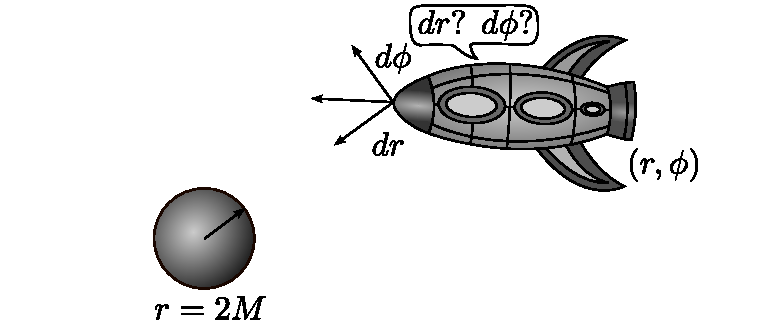
\includegraphics[width=\textwidth]{fig_17-1.pdf}
\captionof{figure}{The spaceship is out of fuel. The engines stop. What will be the next movement in $r$ and $\phi$ direction? \label{fig:stepbystep}}
\end{Figure}

In figure \ref{fig:stepbystep} we show a spaceship at position $(r,\phi,t)$ in \ss coordinates around a black hole of mass $M$. The spaceship has used all its fuel and can therefore not use its engine, it is falling freely. The astronauts in the spaceship are wondering whether the spaceship will pass the black hole so close to the center that they will be swallowed by the black hole or not. We will now study the motion of the spaceship step by step. We will ask the question, what is the new position $(r,\phi,t)$ in \ss coordinates of the spaceship after a time interval $\Delta\tau$ has passed on the wrist watches of the astronauts? We will look for the small increments $\Delta r$, $\Delta\phi$ and $\Delta t$ for each small increment in astronaut proper time $\Delta\tau$. By increasing $\Delta\tau$ and thereby the other coordinates step by step, we will be able to follow the motion $(r,\phi)$ of the spaceship and check if it at some point will reach $r=2M$ or not.

Knowing that the total energy per mass $E/m$ is a constant of motion, we can rewrite the expression
\[
\frac{E}{m}=\sst\frac{dt}{d\tau},
\]
for total energy per mass as
\begin{formbox}
\begin{equation}
\label{eq:t}
\Delta t=\frac{E/m}{\sst}\Delta\tau.
\end{equation}
\end{formbox}
Similarly we can use that the angular momentum per mass $L/m$ is a constant of motion
\[
\frac{L}{m}=r^2\frac{d\phi}{d\tau}
\]
to get
\begin{formbox}
\begin{equation}
\label{eq:phi}
\Delta\phi=\frac{L/m}{r^2}\Delta\tau.
\end{equation}
\end{formbox}
We have already obtained the displacements $\Delta\phi$ and $\Delta t$ per proper time interval $\Delta\tau$. Now we need to find the radial displacement $\Delta r$. The \ss line element (see previous lecture) gives
\[
\Delta s^2=\Delta\tau^2=\sst\Delta t^2-\frac{\Delta r^2}{\sst}-r^2\Delta\phi^2.
\]
We insert the expressions (\ref{eq:t}) and (\ref{eq:phi}) into the line element and obtain
\begin{align*}
&\Delta\tau^2=\\
&\sst\left(\frac{E/m}{\sst}\right)^2\Delta\tau^2-\frac{\Delta r^2}{\sst}\\
&-r^2\left(\frac{L/m}{r^2}\right)^2\Delta\tau^2.
\end{align*}
Reorganizing we find
\begin{formbox}
\begin{equation}
\label{eq:r}
\Delta r=\pm\sqrt{\left(\frac{E}{m}\right)^2-\left[1+\left(\frac{L/m}{r}\right)^2\right]\sst}\Delta\tau.
\end{equation}
\end{formbox}
We now have three equations (\ref{eq:t}), (\ref{eq:phi}) and (\ref{eq:r}) giving us the motion of the spaceship as observed by the far-away observer for each tick $\Delta\tau$ on the wristwatch of the astronauts. Note that these expressions in reality give the first order terms of a Taylor expansion in $\Delta\tau$. The second derivative terms are not included (and will not be treated in this course) and we can therefore not use them in this form to describe a full orbital motion. In orbital motion, when the radial velocity reaches zero, the spaceship will start moving outwards again (do you see that this is the case? Think about the motion of a planet). Radial velocity equal to zero means that the first derivative is zero and that the second derivatives (second order in the Taylor expansion) is needed in order to describe the next step. But we may use it up to the point where the radial velocity is zero. If the radius at this point is outside $r=2M$ we are saved. If the radial velocity does not reach zero before $r=2M$ the spaceship will fall into the black hole. In order to describe the full motion in a more complete manner we can either continue the Taylor expansion to higher orders or, much easier, we can consider the effective potential.

\section{Effective potential}


\begin{Figure}
\centering
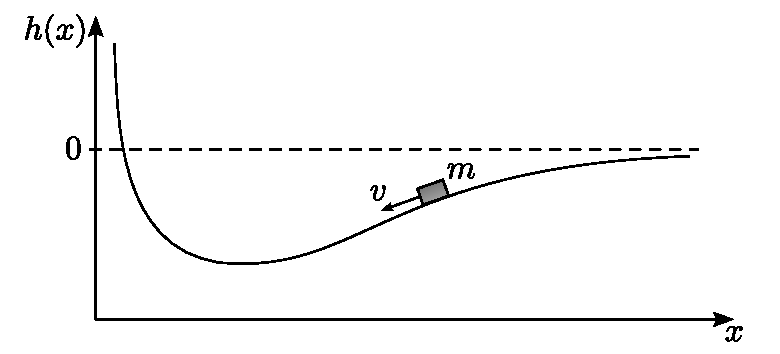
\includegraphics[width=\textwidth]{fig_17-2.pdf}
\captionof{figure}{Object sliding down a frictionless hill with height $h(x)$.\label{fig:fall1}}
\end{Figure}
\begin{Figure}
\centering
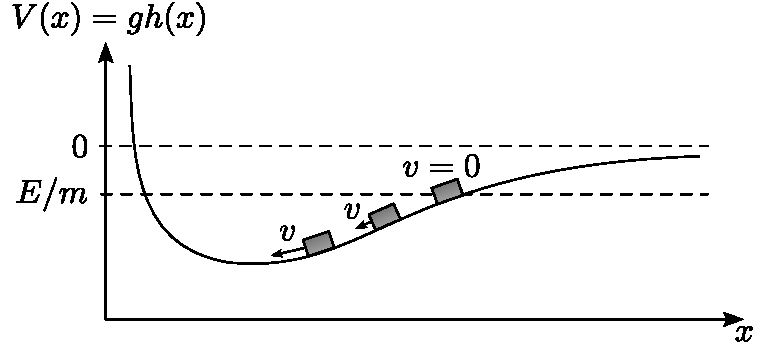
\includegraphics[width=\textwidth]{fig_17-3.pdf}
\captionof{figure}{Object sliding down a frictionless hill with energy per mass $E/m=gh(x)$ deciding the future motion.\label{fig:fall2}}
\end{Figure}



To explain the concept of effective potential, we will go to a well known example: An object sliding down a hill without friction. In figure (\ref{fig:fall1}) we see the situation. An object is located at horizontal position $x$ and at height $h$. We can write the total (Newtonian) energy, kinetic plus potential, with the well known expression
\[
E/m=\frac{1}{2}v^2+gh(x)=\frac{1}{2}v^2+V(x),
\]
where $g$ is the constant gravitational acceleration, $h(x)$ is the height of the hill at position $x$,  $V(x)$ is the potential, $v$ is the velocity of the object and $m$ its mass. In figure \ref{fig:fall2} I have made the same plot as figure \ref{fig:fall1}, but the function is now multiplied by $g$ such that the y-axis now shows $gh(x)$ instead of only $h(x)$. Thus, as you see from the previous expression, the units on the y-axis is now energy per mass and the height of the hill is just the potential $V(x)$. When the velocity is zero $v=0$, the height of the object in this plot directly gives us the total $E/m=gh(x)$ for the object (you can see this from the previous equation: if $v=0$ then $E/m=V(x)$). Thus we can draw a horizontal line passing through this point, showing that this is the energy per mass of the object for all positions $x$ (remember that $E/m$ is constant). The object will have velocity zero at all points where the horizontal line intersects the hill curve (why?).

We have defined the height $h(x)$ to go to asymptotically to zero for large distances $x\rightarrow\infty$. Thus, at large distances the energy of the object consists of purely kinetic energy as the potential energy $gh(x)\rightarrow0$. A total negative energy of the object corresponds to an object left at rest at $h(x)<0$. This object can never reach infinity: We just learned that at infinity the energy of the object is purely kinetic, but kinetic energy cannot be negative. So an object with a negative total energy is trapped in the 'valley' seen in the figures. Note also that an object with negative energy cannot move all the way in to $x=0$, it can only reach up to the point $E/m$ on the y-axis where the velocity will be zero: It will start oscillating back and forth between the two points where the horizontal line at $E/m$ crosses the hill curve. The situation is different for an object with positive energy: Leave the object far out on the positive x axis with an initial velocity different from zero and so large that $E/m$ is positive. By drawing a horizontal line at $E/m$ you can find how far in the object will move before it has $v=0$ from where it will move back an out to infinity. This object is not bound in the valley. The two situations are illustrated in figure \ref{fig:bound} and \ref{fig:free}.

\begin{Figure}
\centering
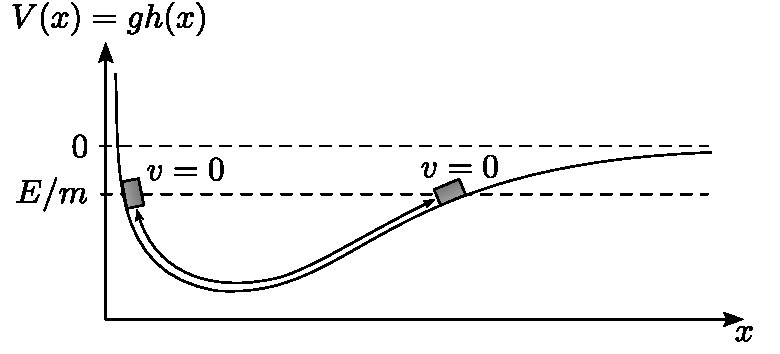
\includegraphics[width=\textwidth]{fig_17-4.pdf}
\captionof{figure}{Bound object oscillating between two points on the hill.\label{fig:bound}}
\end{Figure}
\begin{Figure}
\centering
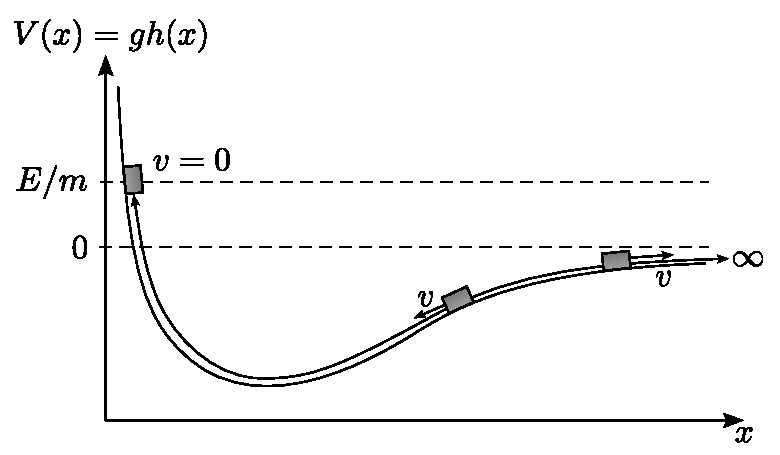
\includegraphics[width=\textwidth]{fig_17-5.pdf}
\captionof{figure}{Free object: slides up to a maximum point and then escapes to infinity.\label{fig:free}}
\end{Figure}


This case was probably not new to you. We will now generalize this situation. We see (from equation \ref{eq:r}) that the equation of motion for this object can be written as
\begin{equation}
\label{eq:general}
A=B\dot{\vec{x}}^2+V(x),
\end{equation}
where $A$ (equal to $E/m$ in our example) and $B$ (equal to $1/2$ in our example) are constants ($B$ being positive), $\vec{x}$ is the position vector of the object and $V(x)$ is the position dependent {\it potential}. If $V(x)$ has a 'valley' similar to figure \ref{fig:fall2} and $V(x)\rightarrow0$ when $x\rightarrow\infty$, then the object with position $\vec{x}$ will move in the following way:
\begin{itemize}
\item With $A<0$ (corresponding to $E<0$ in our example) the object is trapped and will oscillate back and forth between two positions.
\item With $A>0$ (corresponding to $E>0$ in our example), the object can escape out to any position.
\end{itemize}

We recognize the situation described here from a similar physical system: The two body problem. We remember for the two-body problem that an object with negative total energy was bound to orbital motion around the other object whereas objects with positive total energy could escape to infinity. Let's try to see the mathematical analogy. The total energy of an object with mass $m$ close to a star of mass $M$ is
\[
E/m=\frac{1}{2}v^2-G\frac{M}{r},
\] 
and angular momentum
\begin{equation}
\label{eq:spin}
L/m=r^2\dot{\phi}
\end{equation}
using for the moment conventional units. We are only interested in the radial motion of the object, i.e.\ whether the object will be bound or whether it can escape to infinity. We are not interested in the details of the motion in $\phi$ direction. We can rewrite the equation for the energy as
\begin{equation}
\label{eq:newton}
E/m=\frac{1}{2}(\dot{r}^2+r^2\dot{\phi}^2)-G\frac{M}{r}=\frac{1}{2}\dot{r}^2+\left(\frac{1}{2}\frac{(L/m)^2}{r^2}-G\frac{M}{r}\right),
\end{equation}
where equation \ref{eq:spin} was used. Setting $A=E/m$, $B=1/2$ and
\begin{formbox}
\[
V_\mathrm{eff}(r)/m=\frac{1}{2}\frac{(L/m)^2}{r^2}-G\frac{M}{r},
\]
\end{formbox}
we see that equation \ref{eq:newton} can be written on the form of equation \ref{eq:general}. We will call the potential $V(r)$ for the {\it effective potential}. Thus the problem is mathematically identical to the problem of the object sliding down the hill. This means that also the results are identical. The $r$ coordinate corresponds to position on the hill, and the effective potential corresponds to the shape of the hill. In figure \ref{fig:newton} we can see the shape of the 'hill' or effective potential. The object falling in the gravitational field of a star is identical to the object sliding down the hill using the effective potential as the shape of the hill. Again we have the result that for $A=E/m<0$, the object is bound and will oscillate between two $r$ positions which we know (from earlier lectures) are $r=a(1-e)$ and $r=a(1+e)$. Here we have ignored the motion in $\phi$ direction, but we already know that this corresponds to an elliptical orbit. For $E/m=0$, the object will reach zero velocity at in infinite distance $r\rightarrow\infty$. We already learned in previous lectures that this corresponds to the parabolic trajectory. Finally for $E/m>0$, the object can move to infinite distances with arbitrary velocity corresponding to the hyperbolic trajectory. Even though the treatment with effective potential did not give us the exact shape of the orbit it did tell us the essentials using the radial motion only: The object can either oscillate between two radial positions or it can move out to infinity depending on the total energy $E/m$.


\begin{Figure}
\centering
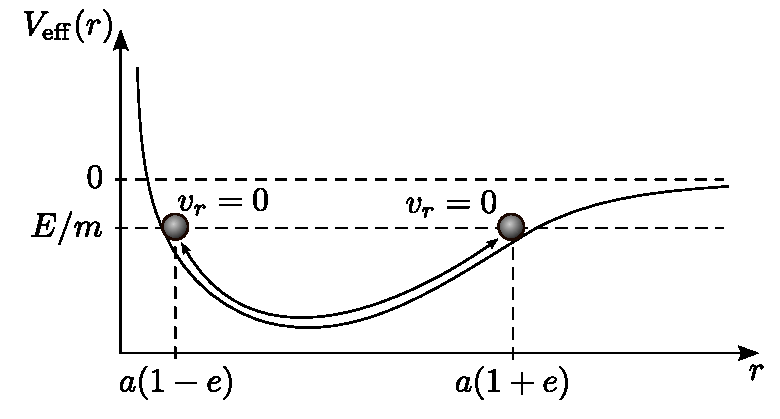
\includegraphics[width=\textwidth]{fig_17-6.pdf}
\captionof{figure}{A bound object in elliptical orbit in a Newtonian effective potential.\label{fig:newton}}
\end{Figure}


\section{Orbital motion in \ss geometry}

We will now turn to the relativistic case. We have seen that by looking just at the radial motion of an object in a gravitational field we can obtain essential information about the future motion of this object without going into details. Equation \ref{eq:r} can be written as
\begin{equation}
\label{eq:rr}
\left(\frac{dr}{d\tau}\right)^2=\left(\frac{E}{m}\right)^2-\left(1-\frac{2M}{r}\right)\left[1+\frac{(L/m)^2}{r^2}\right].
\end{equation}
Again comparing to equation \ref{eq:general} we see that we can make the following substitutions: $A=(E/m)^2$, $B=1$ and
\begin{formbox}
\[
\frac{V_{\rm eff}(r)}{m}=\sqrt{\left(1-\frac{2M}{r}\right)\left[1+\frac{(L/m)^2}{r^2}\right]}
\]
\end{formbox}
We have defined the effective potential such that the square of the effective potential appears in equation \ref{eq:rr}, different from the previous cases. This is just to have an effective potential with units energy. Note that $A$ is now the energy per mass $E/m$ {\it squared} instead of just $E/m$ as we had in the above examples. In equation \ref{eq:general} we only required $A$ to be a constant, it is not required that it equals energy. So we still have exactly the same case as we had above and we can use the same argumentation. Note one more difference: The effective potential goes to $V(r)\rightarrow1$ for large distances instead of $V(r)\rightarrow0$ as above (see the plot of the effective potential in figure \ref{fig:rr}). The reason for this is that the rest energy for a particle in relativistic dynamics is $E/m=1$. If the velocity of the object is zero at large distances then $E/m=1$ whereas in Newtonian dynamics $V(r)\rightarrow0$ because $E/m=0$ at large distances. Remember that in Newtonian dynamics we do not consider the rest energy $E=m$. This makes one difference in our argumentation with respect to above. In the Newtonian case, the limiting energy deciding whether the object would be trapped in the potential and therefore stay in a bound orbit or if it would escape to infinity was $E/m=0$. As we see, in relativistic dynamics this limit is $E/m=1$. If $E/m<1$ then the ball starts falling with zero velocity at some point on the hill below $E/m=1$ and it can therefore never escape to $r\rightarrow\infty$, it will start orbiting. If however the energy $E/m>1$ it has the possibility to escape to infinity as it will have a non-zero velocity as $r\rightarrow\infty$ (check that you understand this by looking at equation \ref{eq:rr} and figure \ref{fig:rr}).


\begin{Figure}
\centering
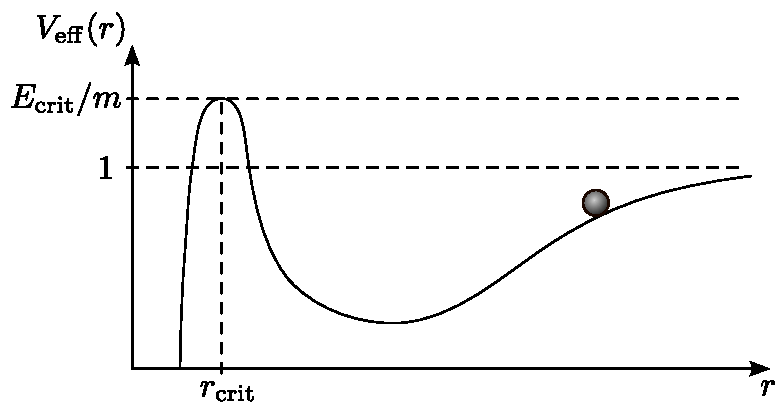
\includegraphics[width=\textwidth]{fig_17-7.pdf}
\captionof{figure}{A bound object in elliptical orbit in a \ss effective potential.\label{fig:rr}}
\end{Figure}

\begin{Figure}
\centering
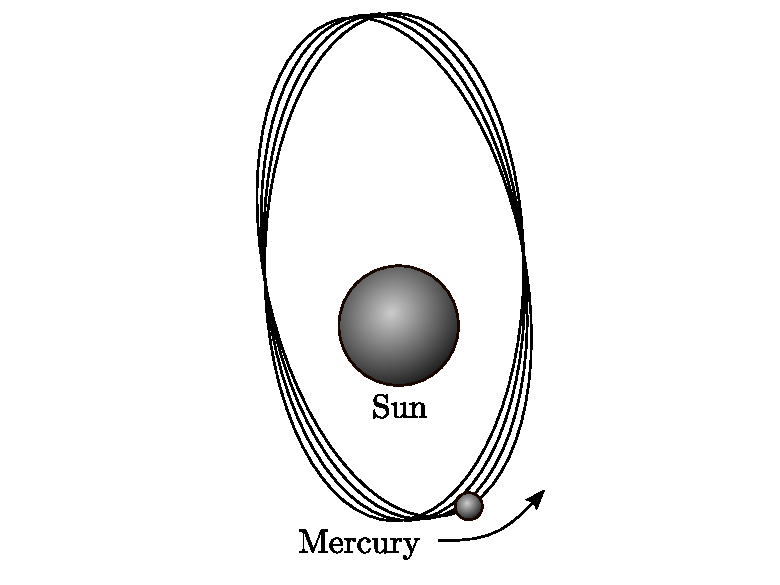
\includegraphics[width=\textwidth]{fig_17-8.pdf}
\captionof{figure}{Perihelion precision of Mercury.\label{fig:peripre}}
\end{Figure}


\begin{figure*}
\fcolorbox{black}{yellow}{\parbox{\dimexpr \linewidth-2\fboxsep-2\fboxrule}{
\begin{minipage}{0.6\textwidth}%{\dimexpr\linewidth-2\fboxsep-2\fboxrule}\parskip=6pt
{\small
\fontfamily{bch}\selectfont
\vspace*{-0.3cm}\hspace*{-0.15cm}\fcolorbox{black}{black}{\bf\color{white} Fact sheet:\color{black}} 
This simulated view based on real data shows stars orbiting the supermassive black hole at the center of the Milky Way along with blue lines marking their orbits. Also, a gas cloud (above center, with its orbit shown in red) has recently been observed approaching the black hole at more than 8 million km/h. The stars and the cloud are shown in their actual positions in 2011. Extremely precise measurements of the stellar orbits in the galactic center show that the supermassive black hole, formally known as Sgr A* (pronounced Sagittarius A star), has a mass of 4.1 million solar masses. The interstellar dust that fills the galaxy blocks our view of the Milky Way's central region in visible light, but astronomers use infrared wavelengths that can penetrate the dust to probe the region.(Figure: ESO)
}
\end{minipage}%\hspace*{0.5cm}
\ \ \ \ \ \ \begin{minipage}{0.35\textwidth}
\centering
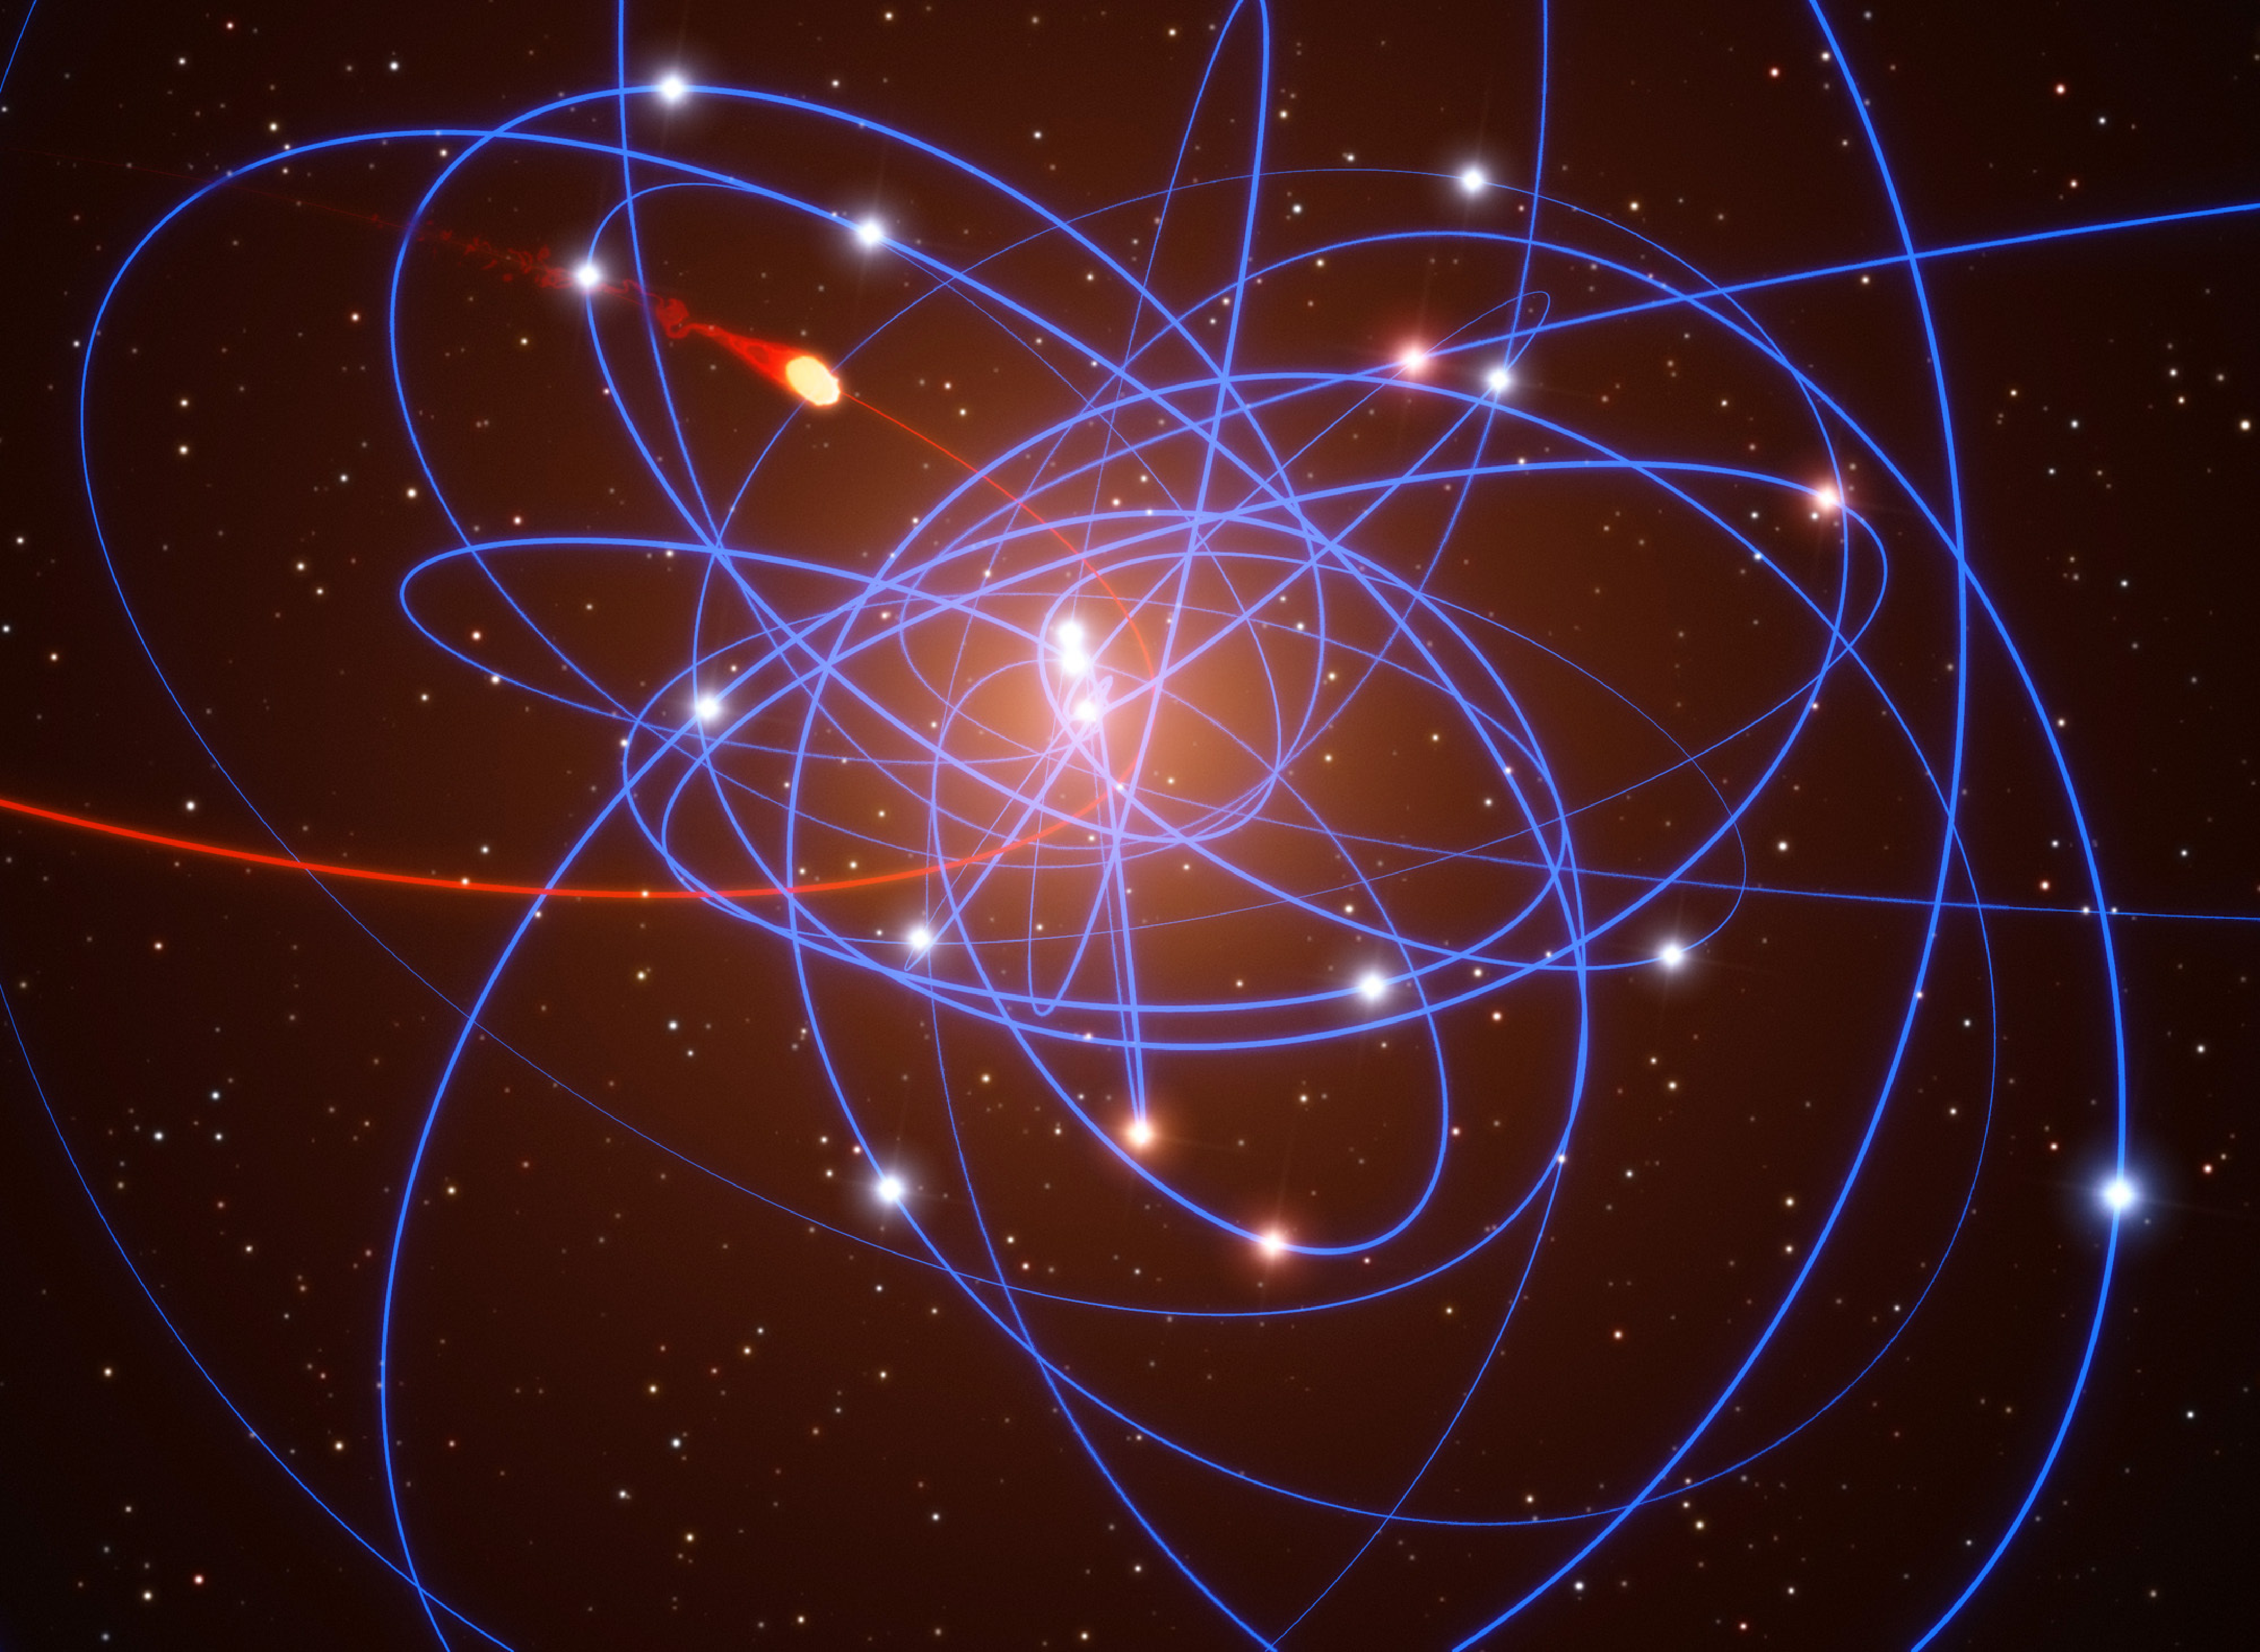
\includegraphics[width=\textwidth]{blackhole_MW_ESO.pdf}
%\end{wrapfigure}
%\end{center}
%\end{figure*}
\end{minipage}
}}
\end{figure*}



Looking at figure \ref{fig:rr} we see one radical difference in the shape of the effective potential with respect to the Newtonian case. At a certain critical radius $r=r_\mathrm{crit}$ the potential has a peak and thereafter it falls steeply downwards towards $r=0$. This is not surprising: Any particle which passes inside the horizon at $r=2M$ cannot escape. We see from figure \ref{fig:rr} that even objects with energies larger than $E/m=1$ (objects which are not bound in the classical sense) may be swallowed by the black hole. The objects with an energy $E/m$ larger than the critical energy $E_\mathrm{crit}/m$ will pass too close to the object, so close that $r<r_\mathrm{crit}$ and it is captured by the black hole. In the Newtonian case, this object would have a large enough energy to escape as $E/m>1$. In the exercises you will derive an expression for $E_\mathrm{crit}$. An object which enters the black hole with an energy $E=E_\mathrm{crit}$ equal the critical energy will make a few orbits around the black hole at $r=r_\mathrm{crit}$ before coincidences will make tiny changes to the energy of the object. These tiny changes may go in either direction, either the object will escape or the object will plunge into the black hole. We thus have three possibilities:
\begin{itemize}
\item $E/m<1$ which gives orbits
\item $1<E/m<E_\mathrm{crit}/m$ for which the object can move to infinity
\item $E/m>E_\mathrm{crit}/m$ for which the object will plunge into the black hole
\end{itemize}

There is one more important difference between the relativistic and the Newtonian effective potential. We will now consider a planet in orbit around a star. Because of the peak at $r=r_\mathrm{crit}$, the potential rises more steeply after the minimum than in the Newtonian case. A planet moving inwards in its orbit towards the star will thus have to climb up this steeper potential and will therefore slow down more close to the perihelion (the point in the orbit of a planet closest to the star). The radial velocity of the planet in the parts of the orbit close to the star is thus slower than in the Newtonian case. Since the planet then spends more time in the orbit close to the star, the planet now also has more time to move in the $\phi$ direction for which there is no slow-down. Thus, in general relativity the planet has moved more in the $\phi$ direction after passing close to the star than it would in the Newtonian case. How does this affect the orbit? The result is that the perihelion moves around the star. This is illustrated in figure \ref{fig:peripre}. For each orbit, the perihelion moves a little bit in $\phi$ direction. In Newtonian physics, the perihelion stays at the same point. This $\phi$ motion of the perihelion is called {\it perihelion precession}.

Long before Einstein discovered the general theory of relativity, it was well known that Mercury, the planet closest to the Sun, had a strong perihelion precession. A large part of this precession could be attributed to the gravitational forces from other planets in the solar system. But the gravitational attraction from other planets was not able to explain the full precession. A little part remained and it turned out that general relativity accounts for exactly this difference.

\section{Inside the horizon}

In the previous lecture we studied an object falling into the black hole from rest at a large distance from the black hole. We found that the conserved energy gave
\[
\sst\frac{dt}{d\tau}=1.
\]
Using this, we obtained the speed of the object as measured by the far-away observer
\[
\frac{dr}{dt}=-\sst\sqrt{\frac{2M}{r}}
\]
and the speed of the object measured by the local shell observers as the object passes the shells
\[
\frac{dr_\sh}{dt_\sh}=-\sqrt{\frac{2M}{r}}.
\]
What is the velocity $dr/d\tau$ measured on the wristwatch time $\tau$ of the falling object? Using these three equations we can write
\begin{equation}
\label{eq:ff}
\frac{dr}{d\tau}=\frac{dr}{dt}\frac{dt}{d\tau}=-\sst\sqrt{\frac{2M}{r}}\sst^{-1}=-\sqrt{\frac{2M}{r}}.
\end{equation}
Even when measuring velocity on the wristwatch of the object, the velocity approaches the speed of light at the horizon and gets larger than the speed of light inside the horizon. But who measures this velocity? Nobody! In this velocity measurement, length is measured by the far-away observer (who cannot measure anything after the object has entered the horizon) and time is measured on the wristwatch of the falling object. We also learned that inside the horizon there are no shell observers to measure the velocity since you cannot be at rest inside the horizon. A local observer sitting in an unpowered spaceship passing the object will always measure that the velocity is less than unity. Why? Because any freely falling observer is in a local inertial frame for a short moment when the spaceship passes nearby, even when inside the horizon. So for the freely falling observer special relativity applies (for a short moment when the spaceship passes nearby)) and he will always measure the velocity of the object as being less than the velocity of light.

How long will it take for the object to reach the singularity in the center from the moment it enters the horizon? We can integrate equation \ref{eq:ff} to find the time measured on the wristwatch of the object
\[
\tau=-\int_{2M}^0dr\sqrt{\frac{r}{2M}}=-\left[\frac{2}{3}\sqrt{\frac{r}{2M}}r\right]_{2M}^0=\frac{4M}{3}.
\]
How long will it take for an observer falling into a black hole with one solar mass to go from the horizon to the singularity? Measured on the wristwatch of the observer it takes
\[
\tau = \frac{4M_\odot}{3} =  \frac{4\times2\times10^{30}{\rm\ kg}\times7.42\times10^{-28}{\rm\ m/kg}}{3} \approx 2000{\rm\ m} \approx 7 {\rm\ \mu s}
\]

% \[
% \tau=\frac{4M_\odot}{3}=\frac{4\times2\times10^{30}{\rm\ kg}\times7.42\times10^{-28}{\rm\ m/kg}}{3}\approx2000{\rm\ m}=\frac{2000{\rm\ m}}{3\times10^8{\rm\ m/s}\approx7{\rm\ \mu s}.
% \]
In problem 3, you will study how the astronaut in a spaceship inside the horizon experiences the world.

\newpage


\TileWallPaper{51.5pt}{11.5pt}{noisy_grid.png}

\section{Problems}

{\bf Problem 1 (2--3 hours)}

\begin{Figure}
\centering
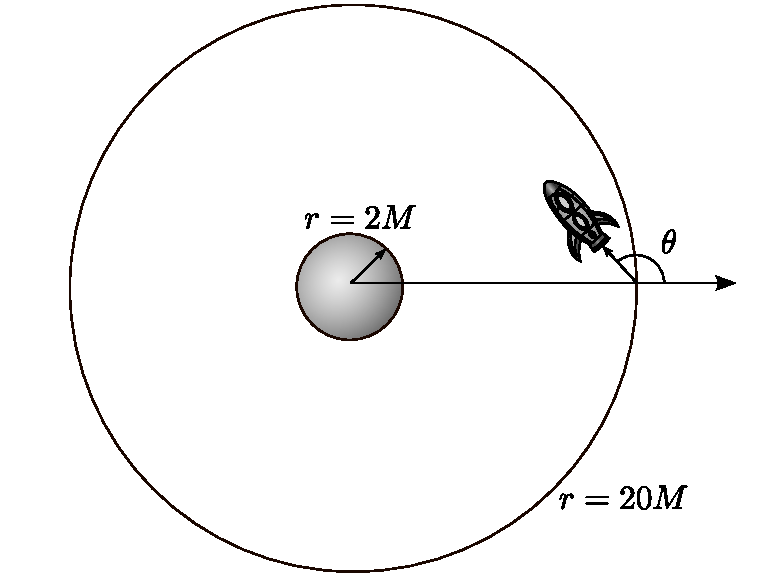
\includegraphics[width=\textwidth]{fig_17-9.pdf}
\captionof{figure}{Rocket launched from shell $r=20M$ inwards at an angle $\theta$. Note: Figure not to scale.\label{fig:rocket}}
\end{Figure}


A rocket is launched from shell $r=20M$ around a black hole of mass $M$ with velocity $v_\sh=0.993$ at an angle $\theta=167^\circ$ with the outward pointing vector from the black hole (see figure \ref{fig:rocket}). Just after launch, there is a problem with the engines and they stop. The shell observers at shell $r=20M$ need to make another rocket to rescue the astronauts, but this takes a long time. The astronauts are worried that they will be captured by the black hole. In this exercise we will try to find out whether the rocket will be captured by the black hole or not. The angular momentum of the rocket is $L$ and the mass of the rocket is $m$. In this exercise you will need the following relation a couple of times
\[
\frac{dx}{d\tau}=\frac{dx}{dt_\sh}\frac{dt_\sh}{d\tau},
\]
where $x$ can be any quantity.
\begin{enumerate}
\item First we need to find out the shape of the effective potential. Use the general relativistic expression for the effective potential to show that the minimum and the maximum of the effective potential are located at the following distances(measured in \ss coordinates) from the black hole
\[
r_\mathrm{extremum}=\frac{(L/m)^2}{2M}\left(1\pm\sqrt{1-\frac{12M^2}{(L/m)^2}}\right).
\]
Which of these two solutions is the maximum of the potential?
\item Show that the angular momentum per mass for the rocket can be written as
\[
\frac{L}{m}=r^2\frac{d\phi}{d\tau}=r\gamma_\sh v_\sh \sin\theta,
\]
where $\gamma_\sh=1/\sqrt{1-v_\sh^2}$.
{\bf Hint 1:} Remember that for short time intervals $dt_\sh$, the shell observers can use special relativity. {\bf Hint 2:} How could we write $dt/d\tau$ in special relativity?
\item Use the general relativistic expression for $E/m$ to show that the total energy per mass of the rocket can be written as
\[
\frac{E}{m}=\sqrt{1-\frac{2M}{r}}\gamma_\sh
\]
\item Insert numbers in the expression for $L/m$ and draw the potential (by hand using the information you have obtained from the previous exercises) having $r$ in units of $M$ on the x-axis and numbers for $V_\mathrm{eff}/m$ on the y-axis.
\item Will the rocket be captured by the black hole?
\item If they are captured by the black hole, how long does it take (on the wristwatch of the astronauts) to reach the singularity from the moment they enter the horizon. For simplicity ignore the spin of the rocket. (give the answer in seconds assuming that this is the black hole in the center of the Milky way, $M\approx4\times10^6M_\odot$). 

{\bf Important hint:} You cannot use the result given in the text. Check that you understand why and find the correct result. In the end you will need to do an ugly integral. Go to 'The Integrator' (\url{http://integrals.wolfram.com/index.jsp}) and type
\[
\verb!1/sqrt(a+b/x)!.
\]

\item What will happen with the astronauts just before entering the singularity? Draw an astronaut and draw the gravitational forces (ok, let's cheat and use forces for a moment since they are easier to draw than spacetime geometry). Which shape will he/she have just before reaching the center?
\end{enumerate}

\vspace{0.5cm}

{\bf Problem 2 (1--2 hours)}

In this exercise we will make a python (or matlab or whatever) code to plot the orbit of the spaceship in the previous exercise. We will start at $r=20M$ and evolve the position of the spaceship forward in time using equations (\ref{eq:phi}), (\ref{eq:r}).
\begin{enumerate}
\item Define variables for $(L/m)/M$ and $(E/m)$ and give them the values you found in the previous exercise. Define a variable for the distance from the black hole $r/M$ and give it the initial value of 20. Finally define a variable $\phi$ which is the angular position with respect to the black hole. We give $\phi$ an initial value of zero. Define a variable which is the number of time steps we will use. Set the variable to 1000. Finally define a variable which is the proper time step $\Delta\tau=0.01$. 
\item Now, define two arrays both with size equal to the number of time steps (1000). The first array will contain the $r$ position at each time step, the other will contain the $\phi$ position at each time step. Set the first element in both arrays to the current value of $r$ and $\phi$.
\item Make a FOR loop over all time steps. For each step, update $r$ and $\phi$ with the increments $\Delta r$ and $\Delta\phi$ until $r/M<2$.
\item Finally we need to plot the orbit. Make two arrays $x$ and $y$ converting the arrays with $r$ and $\phi$ values from polar to Cartesian coordinates. The black hole is at position $x=0$ and $y=0$. Now we have two arrays with the x and y position of the spaceship at different time steps. Now plot a dot at each step in the orbit.
\item Now we will overplot the \ss radius: Make an array with, say 100 elements, with the $r$ position of the horizon $r=2$. Make a corresponding array with equal number of elements having numbers going from 0 to $2\pi$ being the $\phi$ position. Then transform from polar to Cartesian coordinates exactly as you did in the previous step and plot the set of $x$ and $y$ positions you have obtained. Now you will see a circle showing the horizon. 
\item How large angle $\Delta\phi$ did the spaceship revolve around the black hole before entering the horizon?
\end{enumerate}

\vspace{0.5cm}

{\bf Problem 3 (1--2 hours)}

We are in a spaceship inside the horizon falling towards the central singularity. We are trying to find a way to escape. In order to check all possibilities we send one light beam backwards away from the central singularity and one forward towards the central singularity. In order to study how these beams of light are moving we need to write the \ss line element in terms of our wristwatch time $t'$ instead of \ss time $t$. We will make this change of coordinates already before entering the horizon as this allows us to use shell frames as a help. Assume in the following that we have velocity only in the radial direction. Assume also that we started falling freely with velocity $v=0$ far away from the black hole.
\begin{enumerate}
\item Use the Lorentz transformations to show that time intervals measured on the wristwatch of the astronauts are related to time and space intervals measured by shell observers as
\[
dt'=-v_\sh\gamma_\sh dr_\sh+\gamma_\sh dt_\sh,
\]
where $v_\sh$ and $\gamma_\sh$ are based on the local velocity of the astronaut measured by the shell observer at the shell which the spaceship passes. 
\item Use the expressions relating shell coordinates and \ss coordinates to show that
\[
dt'=-\frac{v_\sh\gamma_\sh dr}{\sqrt{\sst}}+\gamma_\sh\sqrt{\sst}dt.
\]
\item In the previous lecture, we deduced the shell velocity $v_\sh$ of a falling spaceship starting with $v=0$ far from the black hole. Go back and check this expression. Insert it in the previous expression and show that
\[
dt=dt'-\frac{\sqrt{2M/r}dr}{\sst}.
\]
\item Use this to substitute $dt$ with $dt'$ in the normal \ss line element and show that the \ss line element can be written
\[
ds^2=d\tau^2=\sst(dt')^2-2\sqrt{\frac{2M}{r}}dt'dr-dr^2-r^2d\phi^2.
\]
Note that this form of the \ss line element does not have a singularity at $r=2M$.
\item We will now study the motion of the two light beams that we emit, one forwards and one backwards. We know that for light, proper time is not moving $d\tau=0$. The light beams in this case are moving only radially so $d\phi=0$. Show that the speed of the two beams can be written as
\[
\frac{dr}{dt'}=-\sqrt{\frac{2M}{r}}\pm1.
\]
After entering the horizon, do the astronauts in the spaceship measure the speed of the light beams to be larger than the speed of light? (think twice before answering)
\item In figure \ref{fig:wl} we show the worldline of the spaceship falling into the black hole. We have also plotted the world lines of light beams emitted from the spaceship at various points in the trajectory. Use the previous equation to explain why the world lines of the light beams look like they do in the figure.
\item What happens to the light beams\ldots in which direction does each of them move? Suppose that the astronauts had a small rescue rocket which could accelerate to a velocity close to the speed of light. They went into the rescue rocket and went in the direction opposite of the black hole. What would happen? How would their motion look like? Do you understand better why nothing can escape the black hole?
\end {enumerate}

\begin{Figure}
\centering
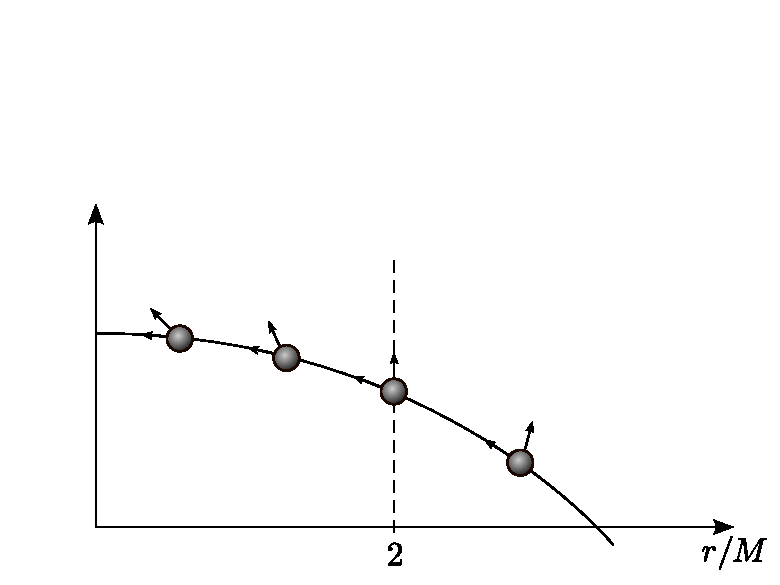
\includegraphics[width=\textwidth]{fig_17-10.pdf}
\captionof{figure}{Worldline of the rocket (marked by a balls) and parts of the worldlines of the forward and backward light beam (arrows) at several points during the free fall into the black hole.\label{fig:wl}}
\end{Figure}


\end{multicols}

\end{document}

